\documentclass[12pt,a4paper]{article}

%% Better math support:
\usepackage{amsmath}

%% Bibliography style:
\usepackage{mathptmx}           % Use the Times font.
\usepackage{graphicx}           % Needed for including graphics.
\usepackage{url}                % Facility for activating URLs.

%% Set the paper size to be A4, with a 2cm margin
%% all around the page.
\usepackage[margin=3cm]{geometry}
\setlength{\parindent}{0em}
%%\setlength{\parskip}{1em}
\renewcommand{\baselinestretch}{1.3}

%% Natbib is a popular style for formatting references.
%%\usepackage{natbib}
%% bibpunct sets the punctuation used for formatting citations.
%%\bibpunct{(}{)}{;}{a}{,}{,}

%% textcomp provides extra control sequences for accessing text symbols:
%%\usepackage{textcomp}
%%\newcommand*{\micro}{\textmu}
%% Here, we define the \micro command to print a text "mu".
%% "\newcommand" returns an error if "\micro" is already defined.

%% This is an example of a new macro that I've created to save me
%% having to type \LaTeX each time.  The xspace command provides space
%% after the word LaTeX where appropriate.
\usepackage{xspace}
%%\providecommand*{\latex}{\LaTeX\xspace}
%% "\providecommand" does nothing if "\latex" is already defined.

%% PATH dos arquivos de imagens
\graphicspath{{../img/}}

%% Suporte ao Idioma Portugues (UTF-8)
\usepackage[portuguese]{babel}
\usepackage[utf8]{inputenc}
\usepackage[T1]{fontenc}

%% Start of the document.
\begin{document}

\author{Clauber Pereira Stipkovic Halic\\
  Universidade Mackenzie\\
  Orientador: Dr. Calebe de Paula Bianchini\\
  Apoio PIVIC Mackenzie}
\date{\today}
\title{COMPUTAÇÃO PARALELA EM JAVASCRIPT}
\maketitle

\section{RESUMO}
\label{sec:section1}

%%\fontsize{10pt}{12pt}\selectfont
JavaScript é a linguagem de programação com maior porcentagem de uso na Web atualmente, por conta da massiva utilização da linguagem em web sites e aplicações ou até mesmo em sistemas operacionais como o Firefox OS da Mozilla, a demanda por rapidez e eficiência de uso de recursos computacionais, faz com as JavaScript Engines sejam cada vez mais exigidas em questão de performance, gerenciamento de memória e uso bateria, e para isso, o interesse em aliar métodos de computação paralela com a linguagem tem aumentando com o passar dos anos. Nesta iniciação científica, apresentamos e definimos a linguagem JavaScript, o funcionamento de uma JavaScript Engine genérica mostrando quais são os passos pelos quais um código JavaScript percorre até ser executado pelo browser, dando ênfase no comportamento da JavaScript Engine da Fundação Mozilla, a SpiderMonkey, atrelada com o modo de funcionamento do Just in Time Compiler. Apresentamos o conceito de computação paralela utilizado atualmente para aplicar recursos como o SIMD e que é implementado por um projeto que tem a finalidade de prover recursos como tipos com os quais é possível utilizar computação paralela para aplicações web através de bibliotecas JavaScript como a SIMD.js que atualmente é desenvolvida por empresas como Mozilla, Google e Intel. \\
Palavras chave: JavaScript; Computação Paralela; SIMD.


\section{ABSTRACT}
\label{sec:section2}

JavaScript is a programming language with the highest percentage of use on the Web today, due to the massive use of the language in websites and applications or even operating systems such as Mozilla's Firefox OS, the demand for speed and resource to an efficiency computer usage, causes an increasingly required of JavaScript Engines in matter of performance, memory management and battery usage, and because of it, the interest in combining methods of parallel computing with the language has increased over the years. This scientific research, presents and defines the JavaScript language, the operation of a generic JavaScript Engine showing what are the steps by which JavaScript code runs to be executed by the browser, emphasizing the JavaScript Engine behavior of the Mozilla Foundation SpiderMonkey, tied with the operation of the JIT Compiler. We are introducing the concept of parallel computing currently used to implement features such as SIMD and which is implemented by a project that aims to provide features such as types with which can be use parallel computing to web applications through JavaScript libraries like SIMD.js which is currently developed by companies like Mozilla, Google and Intel. \\
Keywords: JavaScript; Parallel Computing; SIMD.


\section{INTRODUÇÃO}
\label{sec:section3}

Nos últimos 20 anos, a World Wide Web (conhecida popularmente como Web) se tornou uma ferramenta absolutamente importante para o mundo moderno de modo geral, mudando o modo como o mundo se comunica, executa transações financeiras, aprende entre outras atividades cotidianas, provendo produtos e serviços para suprir essas necessidades, encurtando distancias e facilitando a vida dos usuários. Desde a chamada “guerra dos navegadores”, em meados de 1995, entre os web browsers Microsoft Internet Explorer e Netscape Navigator, quando houve a disputa por mercado entre os dois web browser, o foco dos desenvolvedores de aplicações mudou consideravelmente para acompanhar a transição do foco tipicamente desktop, para o foco multi-device. \\
\\
No início dos anos 90, muitas aplicações eram desenvolvidas apenas e exclusivamente para funcionarem nos desktops; porém, com o passar dos anos, a chegada dos web browsers, e posteriormente, a evolução das linguagem web e dos devices portáteis, fez com que desenvolvedores e empresa ligadas a tecnologia, passassem a ver a web como uma plataforma com imenso potencial para que as aplicações já existentes no desktops, fossem levadas para os web browser, e para que surgissem novas aplicações feitas inteiramente pensando apenas na sua utilização através da web. \\
\\
Com a popularização da internet, a facilidade para adquirir um computador e obter acesso a web, fez com que muitos desenvolvedores e empresas surgissem focadas na criação de aplicações que poderiam ser utilizadas somente pela web. Por volta do ano de 2005, surgiu o conceito de Web 2.0, criado e difundido por Tim O'Reilly, que tinha como objetivo fomentar definitivamente a web como plataforma de desenvolvimento de aplicações, o que abriu espaço para o surgimento de muitos produtos e serviços como leitores de e-mail, aplicações de agências bancarias, etc, que nascer voltados inteiramente para a web, e não mais exclusivamente para desktops. \\
\\
O surgimento de aplicações mais complexas, que utilizam massivamente a linguagem JavaScript, e que demandam recursos computacionais, foi liderado pelo conceito da Web 2.0, o que deu início a preocupação com a velocidade e eficiência de execução de aplicações por parte dos web browsers, tornando as tecnologias que dão suporte a essas aplicações mais importantes com o passar do tempo. \\
\\
Atualmente a linguagem JavaScript não mais executada exclusivamente em web browser, mas também pode ser utilizada para criar aplicações que são executadas no lado servidor, para a escrita de testes de aplicações, entre outras funcionalidades. Todo esse novo ecossistema está disponível através do uso do framework NodeJS, que prove aos desenvolvedores, acesso direto a JavaScript Engine do Google chamada V8. Alem disso, temos esforços da Fundação Mozilla para levar o JavaScript para os dispositivos móveis e smart TVs, criando um sistema operacional baseado inteiramente em tecnologias web com o
Firefox OS.


\section{A LINGUAGEM JAVASCRIPT}
\label{sec:section4}

A linguagem JavaScript foi criada em 1995 pelo desenvolvedor americano, Brendan Eich, como parte do web browser Netscape Navigator, para que este tivesse a habilidade de interpretar scripts do lado cliente, ou seja, os web browsers. \\

\begin{quote}
“JavaScript is a programming language that adds interactivity to your
website (e.g. games, responses when buttons are pressed or data entered in
forms, dynamic styling, animation).” (Mozilla Developer Network)
\end{quote}

David Flanagan (2011) define que JavaScript é uma linguagem de programação dinâmica e multi-paradigma (script, orientada a objetos, imperativa e funcional), conhecida por ser utilizada para interagir com o lado cliente (através da plataforma Document Object Model), comunicação assíncrona e mais atualmente por também haver a possibilidade de ser executada do lado servidor, através do projeto NodeJS. \\
\\
Seu desenvolvimento teve como base a padronização da especificação ECMA-2623 e
ISO/IEC 16262. Ao final de sua implementação a Netscape (atualmente Fundação Mozilla) submeteu em novembro de 1996 a especificação da linguagem JavaScript, que foi aceita e teve a definição do padrão chamada de ECMAScript. A partir de 2012 os browsers mais modernos como Mozilla Firefox, Google Chrome e Opera Browser passaram a dar suporte completo ao ECMAScript 5.1. Em Junho 17 de Junho de 2015, a ECMAScript 6 foi publicada oficialmente e é popularmente chamada pelos desenvolvedores de ES6.

\section{DEFINIÇÃO DE UMA JAVASCRIPT ENGINE}
\label{sec:section5}

Conforme definição apresentada pelo site Mozilla Developer Network, uma JavaScript Engine é “A JavaScript Engine é um interpretador que faz o parsing e executa programas JavaScript.” (tradução), e também é encontrada como JavaScript interpreter ou JavaScript implementation, mas na essência uma JavaScript Engine é uma Virtual Machine (Maquina Virtual). \\
\\
A JavaScript Engine é construída seguindo como base o mesmo princípio de uma virtual machine, e que contem passos que são comuns e definidos para todo tipo de virtual machine:

\begin{itemize}
	\item Parser
	\item Intermediate Representation (IR)
	\item Interpreter
	\item Just-in-Time Compiler / Garbage Collection
	\item Optimization
\end{itemize}

Originalmente, a primeira JavaScript Engine foi construída para possibilitar a execução de código JavaScript no web browser Netscape Navigator, mas atualmente, é utilizada também para execução de códigos JavaScript em CLI (Command Line Interface), o que possibilita utilizar a linguagem também em client-side como ferramenta para automação de tarefas, e até mesmo em aplicações mais robustas onde existe a necessidade de conexões simultâneas com o servidor, onde é utilizado por exemplo, o protocolo WebSocket 	implementado no framework NodeJS.

\subsection{FLUXO DE FUNCIONAMENTO DA JAVASCRIPT ENGINE}
\label{sec:subsection51}

O esquema teórico apresentado na Figura~\ref{fig:figura1}, mostra o fluxo que um código JavaScript percorre na JavaScript Engine, rodando em um processador multi-core, desde recebimento do código até a sua execução. \\

\begin{figure}[h]
	\centering
	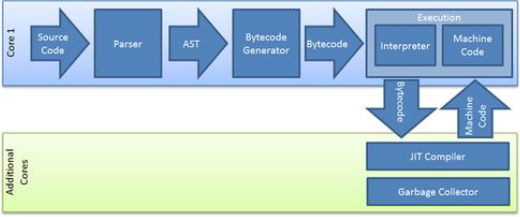
\includegraphics[width=0.7\textwidth]{figura1.png}
	\caption{Esquema lógico sequencial de funcionamento da JavaScript Engine}
	\label{fig:figura1}
\end{figure}

Partindo do início no caminho percorrido pelo código JavaScript, como mostrado no esquema acima, utilizamos um trecho de código que faz uma soma entre dois números e retorna o resultado dessa soma, como prova de conceito para mostrar passo a passo os resultados de cada etapa do processo na JavaScript Engine. O trecho de código pode ser visto na Figura~\ref{fig:figura2}. \\

\begin{figure}[h]
	\centering
	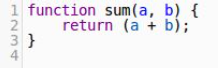
\includegraphics[width=0.3\textwidth]{figura2.png}
	\caption{Código fonte da função "sum"}
	\label{fig:figura2}
\end{figure}

Ao receber o trecho de código, a JavaScript Engine inicia o parsing (conhecido em português como analise sintática), processo que consiste em analisar uma sequência de símbolos ou caracteres em linguagem natural ou de computador, construindo uma estrutura hierárquica correspondente ao que foi informado antes do método de parsing ser aplicado. \\
\\
É durante o processo de parsing também que a validação sintática do código, procurando por possíveis erros baseado na escrita padrão da linguagem é feito, para evitar erros durante a compilação ou resultados divergentes na execução do código ao final do processo. \\
\\
Utilizado a função de soma como exemplo, o resultado do parsing utilizando o método tokenizer\footnote{Tokenizer pode ser um programa que executa analises léxicas em uma sequencia de caracteres.}, temos o resultado do trecho de código da função soma que será gerado e é apresentado na Figura~\ref{fig:figura3}: \\

\begin{figure}[h]
	\centering
	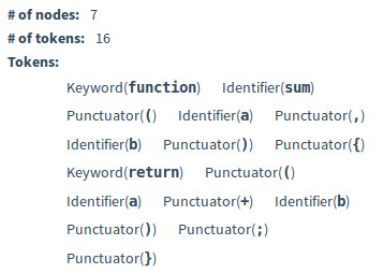
\includegraphics[width=0.4\textwidth]{figura3.png}
	\caption{Resultado do parsing utilizando o método tokenizer}
	\label{fig:figura3}
\end{figure}

Após a geração, uma Abtract Syntax Tree (AST) é formada, como no exemplo para a função de soma conforme mostrado na Figura~\ref{fig:figura4}. \\
\\
Uma vez que a Abstract Syntax Tree é formada, com base no tipo da JavaScript Engine, o bytecode generator converte a Abstract Syntax Tree para uma linguagem intermediaria ou código nativo\footnote{A etapa de geração do bytecode, pode variar nas diferentes implementações de JavaScript Engine, como por exemplo a Rhino \url{https://developer.mozilla.org/en-US/docs/Mozilla/Projects/Rhino/JavaScript_Compiler}, que por ser escrita em linguagem Java, adiciona a etapa de tradução do código JavaScript para classes Java.} , e isso é feito para cada bloco de código dentro da Abstract Syntax Tree. \\
\\
Bytecodes são formas canónicas de representação de códigos (definido no livro do dragão como Intermediate Representation) que são projetados para obter execução eficiente por software interpretador. Assim como muitos interpretadores, uma JavaScript Engine é uma função simples, mas tremendamente longa, que percorre os bytecodes, uma instrução por vez, usando a instrução switch (ou alternativas mais rápidas, dependendo do compilador) para chegar até o ponto apropriado do código para a instrução que será executada. \\
\\
\begin{figure}[h]
	\centering
	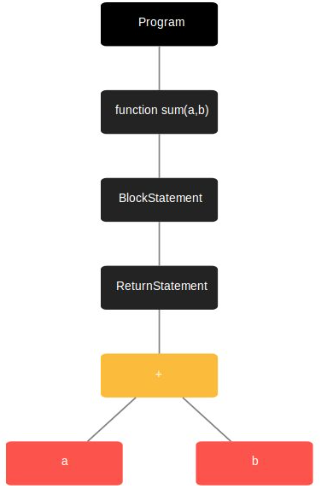
\includegraphics[width=0.4\textwidth]{figura4.png}
	\caption{Abstract Syntax Tree gerada a partir da função "sum", utilizada como exemplo}
	\label{fig:figura4}
\end{figure}

Seguindo o passo de interpretação e compilação na Figura~\ref{fig:figura5}, podemos verificar o bytecode gerado para a função “sum” que utilizamos como referência. \\

\begin{figure}[h]
	\centering
	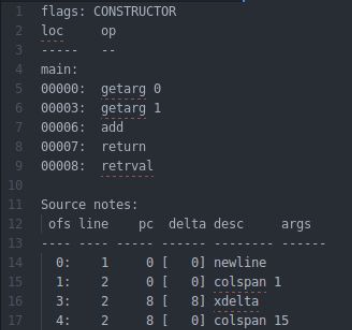
\includegraphics[width=0.4\textwidth]{figura5.png}
	\caption{Bytecode resultante da função "sum"}
	\label{fig:figura5}
\end{figure}

Após a geração do bytecode, entramos na fase de interpretação e execução da representação intermediária, o que é comumente feito utilizando uma função simples, em vários passos, uma instrução por vez percorrendo o bytecode gerado. Quando o bytecode chega até a area de execução, observamos a existência de dois componentes importantes para a performance de uma JS engine, que são o JIT (Just-in-Time Compiler) e o Garbage Collector. \\
\\
O JIT, é responsável por traduzir bytecodes para código de maquina durante a execução do programa, ou seja, assim que um trecho de código é requisitado, o JIT transforma o bytecode para código de maquina, referente ao bloco solicitado e o disponibiliza para execução, fazendo com que a disponibilização do resultado seja rápida e não consuma ciclos de processamento desnecessários entregando somente os blocos que serão utilizados no momento em que forem requeridos. \\
\\
Junto ao JIT, encontramos o Garbage Collector (ou coletor de lixo), que é a área responsável pelo gerenciamento automático da memória que é ocupada por objetos, sendo denominados como “lixo” as posições de memória que estão sendo ocupadas com informações referentes ao programa em execução mas que não são mais relevantes ou que não são mais utilizadas. \\
\\
Tanto o JIT quando o Garbage Collector, são executados quando existe uma solicitação de exibição de um trecho de código JavaScript, e estão disponíveis durante toda a execução da JavaScript Engine, por isso estão diretamente ligados ao passo de execução dentro do processo de interpretação de um código JavaScript.


\section{A JAVASCRIPT ENGINE SPIDERMONKEY}
\label{sec:section6}

Escrita utilizando linguagens de programação como C, C++ e JavaScript, pode ser executado em vários sistemas operacionais e devices como celulares, tablets e até mesmo em aparelho de TV, o que a torna muito adaptável e com robustez e por ser uma JavaScript Engine, a SpiderMonkey\footnote{A JavaScript Engine SpiderMonkey é um projeto de código aberto criado por Brendan Eich, na Netscape Communications em meados de 1996, e é considerada a primeira JavaScript Engine da história.} possui sua estrutura como uma virtual machine e segue um fluxo de interpretação de códigos JavaScript muito próxima ao apresentado no tópico~\ref{sec:subsection51}. \\
\\
Mesmo tendo sua base de construção como sendo uma JavaScript Engine, sua estrutura contem algumas implementações que visam melhorar o desempenho e performance na geração e interpretação de códigos JavaScript, bem como otimizar o gerenciamento e de uso de memória durante o período em que está em execução. \\
\\
Como uma forma de melhorar o desempenho durante a execução do JavaScript, a SpiderMonkey possui duas camadas de JITs que funcionam separadamente e com objetivos diferentes. A primeira camada é conhecida apenas como Baseline Compiler, e que tem como função apenas uma compilação preliminar, ou seja, sem aplicação de análise e otimização do código recebido durante a execução, e foi introduzida para substituir a antiga camada method JIT conhecida como JaegerMonkey, com o objetivo de facilitar a manutenção da JavaScript Engine e por possibilitar a otimização de novas funcionalidades que podem ser criadas nas próximas versões da linguagem JavaScript. \\
\\
A segunda camada, chamada de IonMonkey, foi desenvolvida com foco em performance e otimização na geração do código, sendo inteiramente um method JIT. Essa camada JIT utiliza estratégias diferentes para acelerar e otimizar várias operações. As operações mais comuns e que são relevantes para a execução do programa JavaScript são propriedades e chamadas de função, e passam por uma otimização para obter performance. As estratégias de otimização são classificadas em 5 categorias que são GetProperty, SetProperty, GetElement, SetElement e Call, dentre elas cita-se como exemplo para explicação as estratégias abaixo: \\

\begin{itemize}
	\item GetProperty (obj.prop) – essa otimização só funciona se o objeto de argumentos é usado de maneiras bem definidas dentro da função. A função que contém o argumento é autorizada a utilizar o objeto argumentos.
	\item Call – uma função chamada f(x) envia um frame para a pilha call, seguido de uma chamada, o corpo da função é recebida é copiada, otimizada e devolvida para o frame de execução.
\end{itemize}

Para que seja possível interagir com a JavaScript Engine SpiderMonkey, existe no código fonte uma aplicação chamada de JS Shell, que nada mais é que uma aplicação de CLI que possibilita a execução de funções que acessam diretamente instruções da JavaScript Engine como, por exemplo, obter o resultado bytecode do processo de compilação de um programa JavaScript, e que também é utilizado para a execução de códigos de teste de performance de qualidade da própria SpiderMonkey. \\


\section{A API SIMD.js}
\label{sec:section7}

Em 1966, M. J. Flynn desenvolveu quatro classificações na arquitetura de computadores chamada de taxonomia de Flynn, para descrever modos distintos de entradas e saída de dados que envolvem conceitos de paralelismo. O “Single Instruction, multiple data”, referenciado no livro Introduction to Parallel Processing: Algorithms and Architectures, de Behrooz Parhami(1999) como SIMD Array Processors é uma das quatro classificações da taxonomia de Flynn conhecidas como um caso especial de um programa com um fluxo único de entrada de instruções, múltiplos fluxos de entrada de dados e múltiplas saídas de resultado, chamado de paralelismo de dados, e tem seu fluxo de funcionamento exemplificado na Figura~\ref{fig:figura6}. \\

\begin{figure}[h]
	\centering
	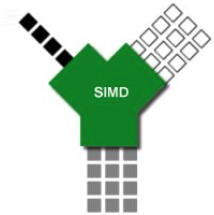
\includegraphics[width=0.4\textwidth]{figura6.png}
	\caption{Esquema de funcionamento da classificação SIMD}
	\label{fig:figura6}
\end{figure}

Utilizando a classificação SIMD, obtém-se um aumento de velocidade substancial em diversas aplicações como gráficos 3D, processamento de imagens e numérico, criptografia entre outras; e se considerarmos a aplicação da SIMD no browser, o aumento de desempenho na utilização de tecnologias como WebGL, Canvas, ASM.js entre outras é significativo e por utilizar poucas instruções para ser executada, a duração de bateria dos aparelhos onde são utilizadas instruções SIMD aumenta consideravelmente. \\
\\
Com foco na web, a interface de programação de aplicações SIMD.js é uma biblioteca JavaScript que esta sendo desenvolvida por empresas como Intel, Google e Mozilla com a intenção de inserir novos tipos e funções paralelas na linguagem JavaScript. Uma das inclusões é referente ao tipo Float32x4, que consiste em representar 4 valores float32, conhecido como Single-precision floating-point format, que podem ser enviados simultaneamente para a JavaScript Engine, pois a SIMD.js possui todas as operações aritméticas básica e operações para rearranjar, carregar e armazenar esses valores. \\
\\
Na biblioteca SIMD.js, existem outros tipos implementados além do tipo Float32x4 (A implementação do tipo Float32x4 segue a especificação 4 IEEE-754 32-bits floating point numbers), conforme mostra a Tabela~\ref{tab:tabela1}: \\

\begin{table}[h]
\begin{center}
\begin{tabular}{|c|c|}
\hline
	Tipo de variável & Especificação técnica do tipo\\
\hline
	int32x4 & 4 32bits Signed Integers \\
\hline
	float64x2 & 2 IEEE-754 64bit Float Point Numbers \\
\hline
	float32x4Array & Array de float32x4 \\
\hline
	int32x4Array & Array de int32x4 \\
\hline
	float64x2Array & Array de float64x2 \\
\hline
\end{tabular}
\caption{Tipos de dados vetoriais da biblioteca SIMD.js}
\label{tab:tabela1}
\end{center}
\end{table}

Observando a hierárquica Figura~\ref{fig:figura7}, apresenta uma relação entre seus objetos JavaScript da biblioteca SIMD.js o esquema se representa da forma como segue: \\

\begin{figure}[h]
	\centering
	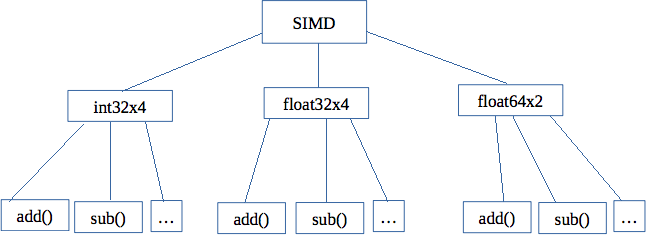
\includegraphics[width=0.7\textwidth]{figura7.png}
	\caption{Hierarquia de objetos da biblioteca JavaScript SIMD.js}
	\label{fig:figura7}
\end{figure}

Utilizando uma aplicação teste feita por Peter Jensen da Intel Corporation, que implementa e renderiza uma representação do o conjunto de Mandelbrot de fractal, percebe-se um ganho de perfomance durante a execução de quase 50\% de frames por segundo (FPS), como mostram as Figura~\ref{fig:figura8} e Figura~\ref{fig:figura9} e os respectivos testes sem a utilização da biblioteca SIMD.js e depois de aplicar a biblioteca JavaScript. \\

Na implementação do teste, quando a execução do script faz uso dos recursos de computação paralela, foram utilizadas duas variáveis com tipos providos pelo SIMD.js, que são SIMD.Int32x4 e SIMD.Float32x4, fazendo com que sejam executadas as operações das funções add(), sub() e mul() simultaneamente para 4 valores informados em cada execução das funções, como pode ser visto se acessado o código fonte do teste. \\

\begin{figure}[h]
	\centering
	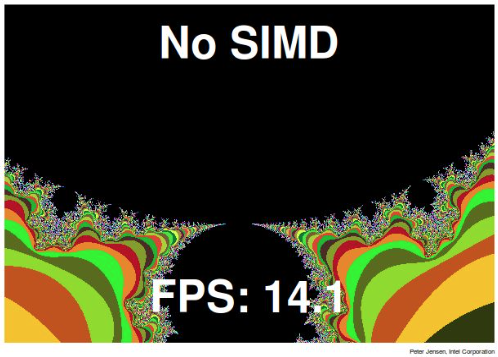
\includegraphics[width=0.4\textwidth]{figura8.png}
	\caption{Renderização do Conjunto de Mandelbrot de fractal - Sem a utilização da SIMD.js}
	\label{fig:figura8}
\end{figure}

\begin{figure}[h]
	\centering
	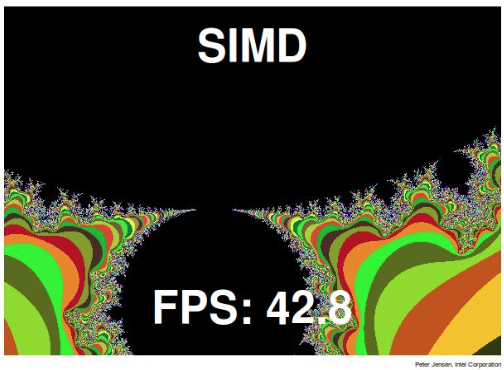
\includegraphics[width=0.4\textwidth]{figura9.png}
	\caption{Renderização do Conjunto de Mandelbrot de fractal - Utilização a SIMD.js}
	\label{fig:figura9}
\end{figure}

Atualmente o foco do desenvolvimento da SIMD.js é suportar tanto arquiteturas x86 com Stream SIMD Extensions quanto arquiteturas ARM com tecnologia NEON.

\newpage
\section{CONCLUSÃO}
\label{sec:section8}

Ao término deste projeto de iniciação científica, percebe-se que existem muitos esforços para que cada vez mais recursos de computação paralela sejam utilização na linguagem JavaScript e que estão partindo de empresas produtoras e consumidoras de tecnologias web, tanto quando de desenvolvedores JavaScript. \\
\\
No caso da JavaScript Engine da Mozilla, a SpiderMonkey, o caminho para a implementação de mais recursos que possam prover funcionalidades de computação paralela já estão caminhando bem por conta da criação de dos dois modos de compilação JIT que essa Engine possui. No caso dos outros browsers como o Google Chrome, por exemplo, a demostração de interesse prover esses recursos é menor, mesmo que esteja envolvida com o projeto citado na pesquisa, o SIMD.js, e no caso da Intel, existe interesse em continuar desenvolvendo e implementando essas novas funcionalidades por ser uma empresas que é envolvida com recursos de hardware e que por conta disso, pode ganhar em qualidade de performance dos web browsers que rodam na plataforma dessa empresa. \\
\\
Com relação as definições da JavaScript Engine e as documentações da Engine SpiderMonkey, observa-se que o desenvolvimento e a documentação desse projetos, sejam publicações acadêmicas ou informais como posts em sites, ainda é muito restrito a um grupo muito pequeno de pessoas que estão realmente envolvidas com desenvolvimento em linguagem C++ e que tem um histórico de envolvimento no desenvolvimento de JIT Compilers, com isso, novos desenvolvedores podem ter uma curva de adaptação e aprendizado muito grande e com isso causar falta de interesse e com essa área. \\
\\
A utilização de recursos de computação paralela como na SIMD.js traz ganhos realmente significativos em relação a performance e utilização de recursos computacionais como por prover melhor utilização dos recursos de processador, pode ser visto no teste feito utilizando conjuntos de Mandelbrot. Muitos outros esforços já estão acontecendo para que mais recursos de computação paralela sejam disponibilizados e utilizados de forma mais objetiva e fácil para os desenvolvedores JavaScript, como por exemplo a especificação ASM.js que esta em desenvolvimento e tem o objetivo de ser um subconjunto de funções para serem utilizadas em JavaScript e a qual tem forte apoio do próprio criador da linguagem, Brendan Eich.

\newpage
\section{BIBLIOGRAFIA}
ACM Digital Library. A LISP garbage-collector for virtual-memory computer system. \\
Disponível em: \url{http://dl.acm.org/citation.cfm?id=363280}. \\
Acesso em: 20 de Maio de 2015. \\
\\
ACM Digital Library. A parallel, real-time garbage collector. \\
Disponível em: \url{http://dl.acm.org/citation.cfm?id=378823}. \\
Acesso em: 20 de Maio de 2015. \\
\\
AHO, Alfred V. et al. Compilers: Principles, Technique, and Tools, Boston, MA: Pearson Education, 2007, 1009 p. \\
\\
ASM.js – Working Draft Specification. \\
Disponivel em: \url{http://asmjs.org/spec/latest/}. \\
Acesso em: 18 de Agosto de 2015. \\
\\
DAHL, Ryan. NodeJS. \\
Disponível em: \url{https://nodejs.org/}. \\
Acesso em: 26 de Abril de 2015. \\
\\
Demo Links with Mandelbrot tests. \\
Disponivel em: \url{http://peterjensen.github.io/idf2014-simd/idf2014-simd.html}. \\
Acesso em: 2 de Agosto de 2015. \\
\\
ECMAScript® 2015 Language Specification, Geneva, CHE: Ecma Internacional, n. 262, junho. 2015. \\
\\
FLANAGAN, David. JavaScript: The Definitive Guide. Sebastopol, CA: O'Reilly Media, 2011. 1096 p. \\
\\
FLYNN, Michael J. Some Computer Organizations and Their Effectivness. IEEE Transactions on Computers. Vol. c-21, No.9, September 1972. \\
Disponível em: \url{http://www.cs.utah.edu/~kirby/classes/cs6230/Flynn.pdf}. \\
Acesso em: 15 de Agosto de 2015. \\
\\
Intel. Parallel JavaScript. \\
Disponível em: \url{https://software.intel.com/enus/blogs/2011/09/15/parallel-javascript}. \\
Acesso em: 10 de Maio de 2015. \\
\\
JavaScript AST Visualizer. \\
Disponível em: \url{http://jointjs.com/demos/javascript-ast}. \\
Acesso em: 10 de Fevereiro de 2015. \\
\\
Jinks, Pete. Anatomy of a Compiler. \\
Disponivel em: \url{http://www.cs.man.ac.uk/~pjj/farrell/comp3.html}. \\
Acesso em: 03 de Março de 2015 \\
\\
Mozilla Developer Network. JavaScript. \\
Disponível em: \url{https://developer.mozilla.org/enUS/docs/Web/JavaScript}. \\
Acesso em: 10 de Dezembro de 2014. \\
\\
Mozilla Developer Network. SpiderMonkey. \\
Disponível em: \url{https://developer.mozilla.org/en-US/docs/Mozilla/Projects/SpiderMonkey}. \\
Acesso em: 27 de Setembro de 2014. \\
\\
NEON – ARM. \\
Disponível em: \url{http://www.arm.com/products/processors/technologies/neon.php}. \\
Acesso em: 13 de Agosto de 2015. \\
\\
O Reilly. What Is Web 2.0: Design Patterns and Business Models for the Next Generation of Software by Tim O'Reilly. \\
Disponível em: \url{http://www.oreilly.com/pub/a/web2/archive/what-isweb-20.html}. \\
Acesso em: 29 de Junho de 2015. \\
\\
PARHAMI, Behrooz. Introduction to Parallel Processing, Santa Barbara, CA: PLENUM SERIES IN COMPUTER SCIENCE, 2002, 532 p. \\
\\
PIENAAR, Jacques A.; HUNDT, Robert. JSWhiz: Static Analysis for JavaScript Memory Leaks. \\
Disponível em: \url{http://static.googleusercontent.com/media/research.google.com/en//pubs/archive/40738.pdf}. \\
Acesso em: 10 de Junho de 2015 \\
\\
SIMD numeric type for EcmaScript. \\
Disponível em: \url{https://github.com/tc39/ecmascript_simd}. \\
Acesso em: 10 de Janeiro de 2015. \\
\\
SpiderMonkey Internal. \\
Disponível em: \url{https://developer.mozilla.org/enUS/docs/Mozilla/Projects/SpiderMonkey/Internals}. \\
Acesso em: 7 de Abril de 2015. \\
\\
Taligarsiel. How browsers work. \\
Disponível em: \url{http://taligarsiel.com/Projects/howbrowserswork1.htm}. \\
Acesso em: 8 de Abril de 2015. \\
\\
TRATT, Laurence. Dynamically Typed Languages. United Kingdom: Advances in Computers, 2009. \\
Disponível em: \url{http://tratt.net/laurie/research/pubs/html/tratt__dynamically_typed_languages/}. \\
Acesso em: 15 de Maio de 2015. \\
\\
The Baseline Compiler Has Landed. \\
Disponivel em: \url{https://blog.mozilla.org/javascript/2013/04/05/the-baseline-compiler-has-landed/}. \\
Acesso em: 10 de Junho de 2015. \\
\\
Wikia. Browser War I. \\
Disponível em: \url{http://browserwars.wikia.com/wiki/Browser_War_I}. \\
Acesso em: 16 de Fevereiro de 2015. \\
\\
W3C. Document Object Model (DOM). \\
Disponível em: \url{http://www.w3.org/DOM/#what}. \\
Acesso em: 7 de Janeiro de 2015. \\
\\
W3C. A Short History of JavaScript. \\
Disponível em: \url{https://www.w3.org/community/webed/wiki/A_Short_History_of_JavaScript}. \\
Acesso em: 15 de Janeiro de 2015. \\

\newpage

\section*{}
Aluno: Clauber Pereira Stipkovic Halic \url{clauber.halic@gmail.com} \\
Orientador: Dr. Calebe de Paula Bianchini \url{calebe.bianchini@mackenzie.br}

\section*{}
\listoffigures
\listoftables

\newpage
\section*{}
\tableofcontents

\end{document}
